\documentclass[tikz,border=6pt]{standalone}
\usepackage{amsmath}
\usepackage{newtxtext,newtxmath}
\usetikzlibrary{arrows.meta,calc}

\begin{document}
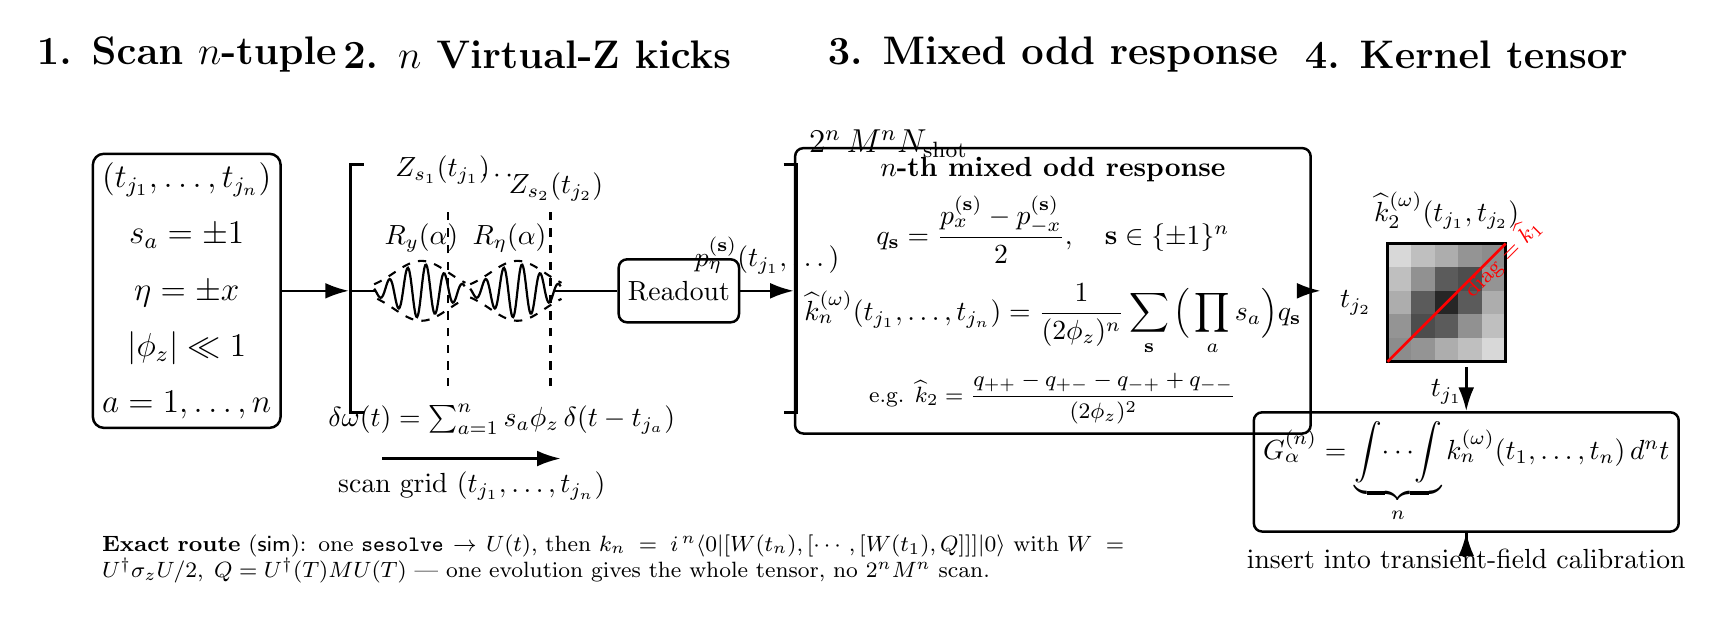
\begin{tikzpicture}[
  x=1cm,
  y=1cm,
  >=Latex,
  font=\large,
  line/.style={draw=black,line width=0.9pt},
  arrow/.style={line,-{Latex[length=3mm,width=2mm]}},
  block/.style={line,rounded corners=3pt,align=center,minimum height=0.8cm},
  smallblock/.style={block,minimum width=1.3cm,font=\normalsize},
  extractbox/.style={line,rounded corners=3pt,align=center,minimum width=5.6cm,minimum height=2.9cm,font=\normalsize},
  setbox/.style={line,rounded corners=4pt,align=center,minimum width=2.15cm,minimum height=2.95cm},
  pulse/.style={line,line width=0.8pt},
  envelope/.style={line,dashed,line width=0.75pt}
]

% Section headings
\node[font=\bfseries\Large] at (1.30,3.35) {1. Scan $n$-tuple};
\node[font=\bfseries\Large] at (5.75,3.35) {2. $n$ Virtual-Z kicks};
\node[font=\bfseries\Large] at (12.30,3.35) {3. Mixed odd response};
\node[font=\bfseries\Large] at (17.55,3.35) {4. Kernel tensor};

% Scan parameters (now an n-tuple of probe times + per-probe signs)
\node[setbox] (scan) at (1.30,0.35)
  {$(t_{j_1},\dots,t_{j_n})$\\[0.22cm]$s_a=\pm1$\\[0.22cm]$\eta=\pm x$\\[0.22cm]$|\phi_z|\ll1$\\[0.22cm]$a=1,\dots,n$};

% Measurement bracket (cost is now 2^n M^n shots)
\draw[line width=1pt]
  (3.55,1.95) -- (3.38,1.95) -- (3.38,-1.20) -- (3.55,-1.20);
\draw[line width=1pt]
  (8.88,1.95) -- (9.05,1.95) -- (9.05,-1.20) -- (8.88,-1.20);
\node[anchor=south west,font=\large] at (9.08,1.92) {$2^{n}\,M^{n} N_{\mathrm{shot}}$};

\draw[arrow] (scan.east) -- (3.36,0.35);
\draw[line] (3.36,0.35) -- (3.7,0.35);

% Pulse sequence, with adjacent Gaussian pulses
\node[font=\normalsize] at (4.28,1.02) {$R_y(\alpha)$};
\begin{scope}[shift={(4.28,0.35)}]
  \draw[pulse,domain=-0.6:0.55,samples=100,smooth]
    plot (\x,{0.34*exp(-5*\x*\x)*sin(deg(27*\x))});
  \draw[envelope,domain=-0.6:0.56,samples=60,smooth]
    plot (\x,{0.38*exp(-4.2*\x*\x)});
  \draw[envelope,domain=-0.56:0.56,samples=60,smooth]
    plot (\x,{-0.38*exp(-4.2*\x*\x)});
\end{scope}

\node[font=\normalsize] at (5.40,1.02) {$R_{\eta}(\alpha)$};
\begin{scope}[shift={(5.5,0.35)}]
  \draw[pulse,domain=-0.6:0.55,samples=100,smooth]
    plot (\x,{0.34*exp(-5*\x*\x)*sin(deg(27*\x))});
  \draw[envelope,domain=-0.6:0.56,samples=60,smooth]
    plot (\x,{0.38*exp(-4.2*\x*\x)});
  \draw[envelope,domain=-0.6:0.56,samples=60,smooth]
    plot (\x,{-0.38*exp(-4.2*\x*\x)});
\end{scope}

% Multiple Virtual-Z insertions at the n scanned times (n=2 shown)
\draw[line,dashed] (4.62,-0.86) -- (4.62,1.36);
\node[font=\normalsize,anchor=south] at (4.55,1.58) {$Z_{s_1}(t_{j_1})$};
\draw[line,dashed] (5.92,-0.86) -- (5.92,1.36);
\node[font=\normalsize,anchor=south] at (5.99,1.36) {$Z_{s_2}(t_{j_2})$};
\node[font=\normalsize] at (5.27,1.80) {$\cdots$};
\node[font=\normalsize,anchor=north] at (5.30,-0.96)
  {$\delta\omega(t)=\textstyle\sum_{a=1}^{n}s_a\phi_z\,\delta(t-t_{j_a})$};

% Scan direction marker: the full n-dimensional grid of probe times
\draw[arrow] (3.78,-1.78) -- (6.05,-1.78);
\node[font=\normalsize,anchor=north] at (4.92,-1.82)
  {scan grid $(t_{j_1},\dots,t_{j_n})$};

\node[smallblock,minimum width=1.1cm] (readout) at (7.55,0.35) {Readout};
\draw[line] (5.96,0.35) -- (readout.west);

% Mixed-difference extraction (n-th mixed partial; n=2 written out)
\node[extractbox] (extract) at (12.30,0.35)
  {\textbf{$n$-th mixed odd response}\\[0.14cm]
   $q_{\mathbf{s}}=\dfrac{p_x^{(\mathbf{s})}-p_{-x}^{(\mathbf{s})}}{2},\quad \mathbf{s}\in\{\pm1\}^{n}$\\[0.22cm]
   $\widehat{k}_n^{(\omega)}(t_{j_1},\dots,t_{j_n})=
   \dfrac{1}{(2\phi_z)^{n}}\displaystyle\sum_{\mathbf{s}}\Big(\prod_{a}s_a\Big)q_{\mathbf{s}}$\\[0.20cm]
   {\footnotesize e.g. $\widehat{k}_2=\dfrac{q_{++}-q_{+-}-q_{-+}+q_{--}}{(2\phi_z)^2}$}};
\draw[arrow] (readout.east) -- node[above,font=\normalsize,pos=0.50,yshift=0.08cm]
  {$p_{\eta}^{(\mathbf{s})}(t_{j_1},\dots)$} (extract.west);

% Kernel tensor: 2-D heatmap (n=2) with diagonal = 1-D kernel
\begin{scope}[shift={(16.55,-0.55)}]
  \def\cs{0.30}
  \foreach \i in {0,...,4}{
    \foreach \k in {0,...,4}{
      \pgfmathsetmacro{\op}{min(1,0.55*exp(-0.16*((\i-2)^2+(\k-2)^2))+0.30*exp(-0.55*((\i-\k)^2)))}
      \fill[black,opacity=\op] (\i*\cs,\k*\cs) rectangle (\i*\cs+\cs,\k*\cs+\cs);
    }
  }
  \draw[line] (0,0) rectangle (5*\cs,5*\cs);
  \draw[red,line width=1pt] (0,0) -- (5*\cs,5*\cs);
  \node[font=\normalsize,anchor=north] at (2.5*\cs,-0.10) {$t_{j_1}$};
  \node[font=\normalsize,anchor=east] at (-0.08,2.5*\cs) {$t_{j_2}$};
  \node[font=\normalsize,anchor=south] at (2.5*\cs,5*\cs+0.06)
    {$\widehat{k}_2^{(\omega)}(t_{j_1},t_{j_2})$};
  \node[red,font=\footnotesize,anchor=west,rotate=45] at (3.05*\cs,2.65*\cs)
    {diag $=\widehat{k}_1$};
\end{scope}

% Multi-dimensional integral (kernel "volume")
\node[block,minimum width=5.0cm,minimum height=1.0cm,font=\normalsize] (area) at (17.55,-1.95)
  {$G_\alpha^{(n)}=\underbrace{\int\!\cdots\!\int}_{n}
   k_n^{(\omega)}(t_1,\dots,t_n)\,d^{n}t$};
\draw[arrow] (extract.east) -- (15.70,0.35);
\draw[arrow] (17.55,-0.62) -- (area.north);

\node[font=\normalsize,align=center] at (17.55,-3.05)
  {insert into transient-field calibration};
\draw[arrow] (area.south) -- (17.55,-2.72);

% Footnote: the exact/cheap route avoids the 2^n M^n scan
\node[font=\footnotesize,align=left,anchor=north west,text width=13.6cm] at (0.10,-2.62)
  {\textbf{Exact route} (\textsf{sim}): one $\mathtt{sesolve}\!\to\!U(t)$, then
   $k_n=i^{\,n}\langle0|[W(t_n),[\cdots,[W(t_1),Q]]]|0\rangle$ with
   $W=U^{\dagger}\sigma_z U/2,\;Q=U^{\dagger}(T)MU(T)$ --- one evolution gives
   the whole tensor, no $2^{n}M^{n}$ scan.};

\end{tikzpicture}
\end{document}
